\subsection{Data Likelihood} \label{sec:likelihood}

As data we consider here the positions and velocities of stars coming from a given \MAP{} and survey selection function $\text{sf}(\vect{x})$,
\begin{eqnarray*}
D  =\{ \vect{x}_i,\vect{v}_i \mid && \text{(star $i$ belonging to same \MAP{})}\nonumber\\
&\wedge& (\text{sf}(\vect{x_i}) > 0) \}.
\end{eqnarray*}

The model that we fit is specified by a number of fixed and free parameters,
\begin{eqnarray*}
\pmodel =\{ p_\text{DF} , p_\Phi \}.
\end{eqnarray*}
For the qDF parameters (see Section \ref{sec:qDF}) we assume a prior that is flat in
\begin{eqnarray}
p_\text{DF} := \{ \ln h_R, \ln \sigma_{R,0}, \ln \sigma_{z,0}, \ln h_{\sigma,R}, \ln h_{\sigma,z} \}.\label{eq:p_DF}
\end{eqnarray}
The orbit of the $i$-th star in a potential with $p_\Phi$ is labeled by the actions $\vect{J}_i := \vect{J}[\vect{x}_i,\vect{v}_i\mid p_{\Phi}]$ and the qDF evaluated for the $i$-th star is then $\text{qDF}(\vect{J}_i \mid \pmodel) := \text{qDF}(\vect{J}[\vect{x}_i,\vect{v}_i\mid p_{\Phi}] \mid p_\text{DF})$.\\

The likelihood of the data given the model is
\begin{eqnarray}
&&\mathscr{L}(D \mid \pmodel) \nonumber\\
&&\equiv \prod_i^{N} p(\vect{x}_i,\vect{v}_i \mid \pmodel) \nonumber\\
&&= \prod_i^{N} \frac{\text{qDF}(\vect{J}_i \mid \pmodel) \cdot \text{sf}(\vect{x}_i)}{\int \Diff 3 x \Diff 3 v \  \text{qDF}(\vect{J} \mid \pmodel) \cdot \text{sf}(\vect{x})}\nonumber\\
&&\propto \prod_i^{N} \frac{\text{qDF}(\vect{J}_i \mid \pmodel)}{\int \Diff 3 x \  \rho_\text{DF}(R,|z| \mid \pmodel) \cdot \text{sf}(\vect{x})}, \label{eq:prob}
%\label{eq:likelihood}
\end{eqnarray}
where $N$ is the number of stars in the data set $D$, and in the last step we used Equation \ref{eq:tracerdensity}. The factor $\prod_i\text{sf}(\vect{x}_i)$ is independent of the model parameters so we treat it as unimportant proportionality factor in the likelihood calculation. We find the best set of model parameters by maximizing the posterior probability distribution $\pdf{}(\pmodel \mid D)$, which is according to Bayes' theorem proportional the likelihood $\mathscr{L}(D\mid \pmodel)$ times the prior. We assume flat priors in both $p_\Phi$ and $p_\text{DF}$ (see Equation \ref{eq:p_DF}) through out this work, then \pdf{} and likelihood can and will be used interchangeably for the remainder of the work.\\

The normalisation in Equation \ref{eq:prob} is a measure for the total number of tracers inside the survey volume,
\begin{equation}
M_\text{tot} \equiv \int \Diff 3 x \  \rho_\text{DF}(R,|z| \mid \pmodel) \cdot \text{sf}(\vect{x}).\label{eq:normalisation}
\end{equation}
In the case of an axisymmetric galaxy model and $\text{sf}(\vect{x})=1$ everywhere inside the observed volume (i.e. a complete sample as assumed in most tests in this work), the normalisation is essentially a two-dimensional integral in $R$ and $z$ of the interpolated tracer density $\rho_{DF}$ in Equation \ref{eq:tracerdensity} over the differential survey volume, i.e. $\frac{\partial M_\text{tot}}{\partial \phi} (R,z) = \int \diff R \ \diff z \ \rho_\text{DF} \times \frac{\partial V}{\partial \phi}$ \Jo{[TO DO: missing factor of R???]}. We perform this integral as a Gauss Legendre quadrature of order 40 in each $R$ and $z$ direction. The angular integral, i.e. $M_\text{tot} = \int R \diff \phi \ \frac{\partial M_\text{tot}}{\partial \phi}$, can be solved analytically. 
\\It turns out that the sufficiently accurate evaluation of the likelihood is computationally expensive, even for only one set of model parameters. This expense is dominated by the number of action calculations required, which in turn depends on the number of stars in the sample and the numerical accuracy of the integrals in Equation \ref{eq:tracerdensity} needed for the normalisation, which requires $N_x^2 \times N_v^3$ action calculations. The accuracy has to be chosen high enough, such that a resulting numerical error 
\begin{equation}
\delta_{M_{tot}} \equiv \frac{M_\text{tot,approx}(N_x,N_v,N_\sigma) -  M_\text{tot} }{M_\text{tot}}\label{eq:relerrlikelihood}
\end{equation}
\Wilma{[TO DO: make sure every Mtottrue is replaced by Mtot]}
does not dominate the likelihood, i.e.
\begin{eqnarray}
& &\log \mathscr{L}(\pmodel \mid D) \nonumber\\
&& = \sum_i^{N} \log \text{qDF}(\vect{J_i} \mid \pmodel) - 3N \log \left( r_o v_o\right)\nonumber\\
& & -N \log(M_\text{tot}) - N \log (1 + \delta_{M_{tot}}),\label{eq:loglikelihood_relerr}
\end{eqnarray}
with
\begin{eqnarray}
N \log (1 + \delta_{M_{tot}}) \lesssim 1.\nonumber
\end{eqnarray}
In other words, this error is only small enough if it does not affect the comparison of two adjacent models whose log-likelihoods differ, to be clearly distinguishable, by 1. Otherwise numerical inaccuracies could lead to systematic biases in the potential and DF fitting. For data sets as large as $N =$ 20,000 stars, which in the age of Gaia could very well be the case \HW{[TO DO: Really???]}, one needs a numerical accuracy of 0.005\% in the normalisation. Figure \ref{fig:norm_accuracy} demonstrates that the numerical accuracy we use in the analysis, $N_x=16$, $N_v=24$ and $N_{sigma}=5$, does satisfy this requirement.\\

%====================================================================

%FIGURE: accuracy in the likelihood normalisation 

\begin{figure*}
\centering
\plotone{figs/normalisation_accuracy_4.eps}
\caption{Relative error  $\delta M_\text{tot}$ of the likelihood normalization $M_\text{tot}$ in Equation \ref{eq:relerrlikelihood} depending on the accuracy of the grid-based density calculation in Equation \ref{eq:tracerdensity} (and surrounding text). We show how $\delta M_\text{tot}$ varies with the spatial resolution (first column), velocity resolution (second column) and velocity integration range (third column) for two different potentials (\texttt{KKS-Pot} in the first row and \texttt{MW13-Pot} in the second row) and five different spherical observation volumes with radius $r_\text{max}$ (color coded according to the legend). (Test \ref{test:norm_accuracy} in Table \ref{tbl:tests} summarizes all model parameters.) $N_x$ is the number of spatial grid points in $R \in R_\odot \text{kpc} \pm r_\text{max}$ and $|z| \in [0,r_\text{max}]$ on which the density is evaluated according to Equation \ref{eq:tracerdensity}. The spatial resolution in $z$ is therefore $r_\text{max}/N_x$ and $2r_\text{rmax}/N_x$ in $R$. This choice is reasonable because the density is symmetric in $z$ and varies less in $R$ than in $z$, because the tracer scale length of the disk is much larger than its scale height. At each $(R,z)$ of the grid a Gauss-Legendre integration of order $N_v$ is performed over an integration range of $\pm n_\sigma$ times the velocity dispersion in $v_R$ and $v_z$ and $[0,1.5v_\text{circ}(R_\odot)]$ in $v_T$. $n_\sigma/N_v$ is therefore a proxy for the velocity resolution of the grid. (We vary $N_x$, $N_v$ and $n_\sigma$ separately and keep the other two fixed at the values indicated above the columns.) To arrive at the approximation $M_\text{tot,approx}$ for $M_\text{tot}$ in Equation \ref{eq:normalisation}, we perform a 40th-order Gauss-Legendre integration in each $R$ and $z$ direction of the interpolated density over the observed volume. We calculate the ``true'' normalization with high accuracy as $M_\text{tot} \approx M_\text{tot,approx}(N_x=20,N_v=56,N_\sigma=7)$. The black dots indicate the accuracy used in our analyses: It is better than $0.002\%$. Only for the smallest volume in the \texttt{MW13-Pot} (yellow line) the error is only $\sim 0.005\%$. This could be due to the fact, that, while we have analytical formulas to calculate the actions for the Staeckel potential \texttt{KKS-Pot} exactly, we have to resort to an approximate action calculation for the MW-like potential \texttt{MW13-Pot} (see Section \ref{sec:potentials}). \Wilma{[TO DO: Write $|\delta M_\text{tot}|$ on y-axis] [TO DO: Remove MW13-Pot completely from this plot, caption and test table] [TO DO: Caption too long] [TO DO: Rewrite caption, text and table, I changed the plot]}}
\label{fig:norm_accuracy}
\end{figure*}


%====================================================================
\Wilma{[TO DO: Comment by HW: What I am missing in this Section is any distinction of what aspects are "new" (not addressed in existing papers) and what is recapitulated to be coherent.]}

If the data is affected by measurement errors, they have to be incorporated in the likelihood. We assume Gaussian errors in the observable space $\vect{y} \equiv (\tilde{\vect{x}},\tilde{\vect{v}})=(\text{RA},\text{DEC},(m-M),\mu_\text{RA},\mu_\text{DEC},v_\text{los})$, i.e. the $i$-th star's observed $\vect{y}_i \sim N[{\vect{y}'}_i,\delta \vect{y}_i](\vect{y}) = N[\vect{y},\delta \vect{y}_i]({\vect{y}'}_i)$ \HW{[TO DO: Talk to HW about best notation.]}, with ${\vect{y}_i}'$ being the true position and velocity of the star. Stars follow the (quasi-isothermal) distribution function (DF$(\vect{y}') \equiv$ qDF$(\vect{J}[\vect{y}' \mid p_\Phi] \mid p_\text{DF})$ for short), convolved with the error distribution $N[0,\delta \vect{y}](\vect{y}')$ \Wilma{[TO DO: CHECK AGAIN]}. The selection function sf$(\vect{y})$ acts on the space of (error affected) observables. 
Then the probability of one star becomes
\begin{eqnarray*}
&&\tilde{p}(\vect{y}_i \mid p_\Phi,p_\text{DF},\delta \vect{y}_i)\\
& \equiv& \frac{\text{sf}(\vect{y}_i) \cdot \int \Diff{6} y' \  \text{DF}(\vect{y}') \cdot N[\vect{y}_i,\delta \vect{y}_i](\vect{y}')}{\int \Diff{6}y'  \  \text{DF}(\vect{y}')  \cdot  \int \Diff{6} y \  \text{sf}(\vect{y})  \cdot N[\vect{y}',\delta \vect{y}_i](\vect{y})}.
\end{eqnarray*}
In the case of errors in distance or position, the evaluation of this is computational expensive - especially if the stars have heteroscedastic errors $\delta \vect{y}_i$, for which the normalisation would have to be calculated for each star separately. In practice we apply the following approximation,
\begin{eqnarray}
&&\tilde{p}(\vect{y}_i \mid p_\Phi,p_\text{DF},\delta \vect{y}_i) \nonumber\\
&\approx& \frac{ \text{sf}(\vect{x}_i)}{\int \Diff{6}y'  \  \text{DF}(\vect{y}')  \cdot   \text{sf}(\vect{x}')} \cdot \frac{1}{N_\text{error}} \sum_n^{N_\text{error}}  \text{DF}(\vect{x}_i,\vect{v}[\vect{y}'_{i,n}]) \label{eq:errorconv}
\end{eqnarray}
with
\begin{eqnarray}
\vect{y}'_{i,n} \sim N[\vect{y}_i,\delta \vect{y}_i](\vect{y}')\nonumber
\end{eqnarray}
In doing so, we ignore errors in the star's \HW{position $\vect{x}_i$ [TO DO: something is not clear to HW here]} altogether. This simplifies the normalisation drastically and makes it independent of measurement errors, including the velocity errors. \HW{Distance errors however are included [TO DO: something is not clear to HW here]}, but only implicitly in the convolution over the stars' velocity errors in the Galactocentric rest frame. We calculate the convolution using Monte Carlo integration with $N_\text{error}$ samples drawn from the full error Gaussian in observable space, $y'_{i,n}$. 
\\Figure \ref{fig:isoSphFlexErrConv_MC_vs_error} demonstrates that in the absence of distance errors the $N_\text{error}$ needed for the convolution integral to converge depends as
\begin{equation*}
N_\text{error} \propto \delta v^2
\end{equation*}
on the uncertainties in the (1D) velocities.

%=============================================================

\begin{figure}
\centering
\subfigure[$N_* = 10,000$]{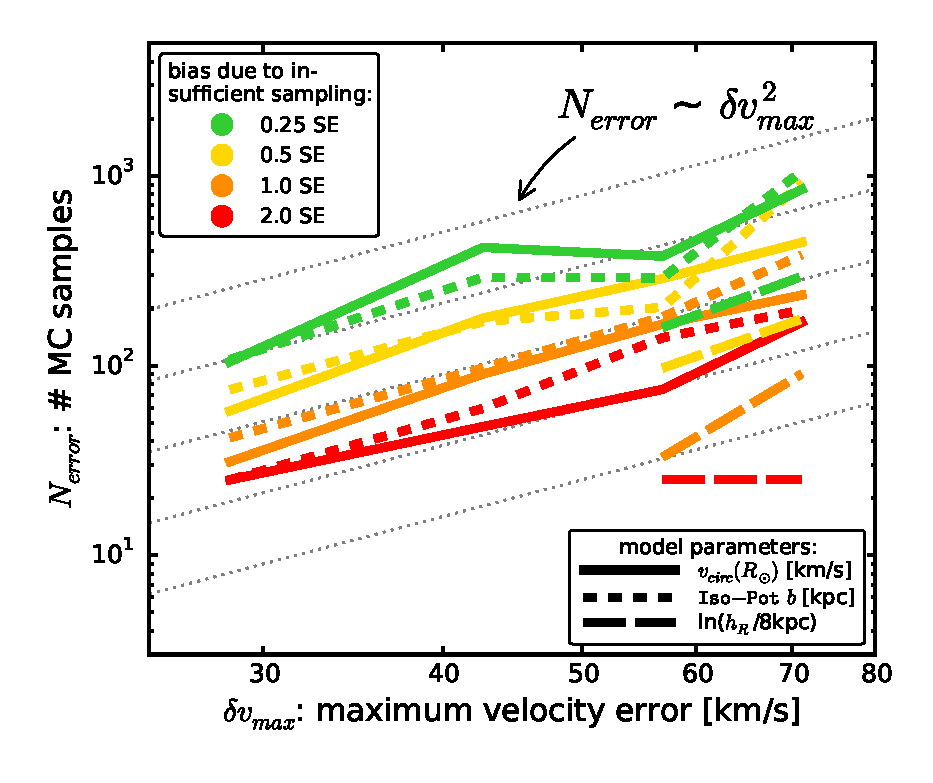
\includegraphics[width=60mm]{figs/isoSphFlexErrConv_MC_vs_error_2.eps}}
\subfigure[$N_* = 5,000$]{
\includegraphics[width=60mm]{figs/Coming-Soon-Placeholder.eps}}
\caption{Number of Monte Carlo (MC) samples $N_\text{error}$ needed for the numerical convolution of the model probability with the measurement uncertainties in Equation \ref{eq:errorconv}, given the maximum velocity error $\delta v_\text{max}$ within the stellar sample. Unsufficent sampling introduces systematic biases in the parameter recovery as indicated in the legend. The relation found here, $N_\text{error} \propto \delta v_\text{max}^2$, was distilled from a set of analyses of mock data sets with different proper motion uncertainties $\delta \mu \in [2,5]~\text{mas yr}^{-1}$ in the absence of distance errors (see Test \ref{test:isoSphFlexErrConv_MC_vs_error} in Table \ref{tbl:tests}). The proper motion error $\delta \mu$ translates to heteroscedastic \Wilma{[TO DO: make sure that this word is written correctly everywhere.]} velocity errors according to $\delta v [\text{km s}^{-1}] \equiv 4.74047 \cdot r[\text{kpc}] \cdot \delta \mu [\text{mas yr}^{-1}]$, with $r$ being the distance of the star from the Sun. Stars with larger $\delta v$ require more $N_\text{error}$ for the integral over its measurement uncertainties to converge. We therefore show how the $N_\text{error}$ needed for the potential \pdf{} of the whole data set to be converged, depends on the largest velocity error $\delta v_\text{max} \equiv \delta v(r_\text{max})$ within the data set. We used $N_\text{error} = 800$ and  $1200$ for $\delta \mu \leq 3 \text{mas yr}^{-1}$ and $\delta \mu > 3 \text{mas yr}^{-1}$, respectively, as the reference for the converged convolution integral (see also left panels in Figure \ref{fig:isoSphFlexErrConv_bias_vs_SE}). \Wilma{[TO DO: some of the 25 MC sample analyses have to be re-done.] [TO DO: Replace right plot with new plot with $N_* = 5,000$] [TO DO: Use $N_*$ everywhere where applicable] [TO DO: Intriduce $N_*$ somewhere.] [TO DO: Iso-Pot in legend]} \Wilma{[TO DO: Comment from Jo: I think it is important to test, if the MC vs error plot depends on number pf stars. Maybe test it with less stars (5000), to test this quickly. Naively, I would expect a large depedence on Ndata.]}}
\label{fig:isoSphFlexErrConv_MC_vs_error}
\end{figure}

%=============================================================